\scanpage{105}
$s\in\widetilde E_a$ définit
\[
\begin{aligned}
\widetilde E_b&\overset{f_{s,b}}{\simeq}E_b\times\{\pm1\}
&\qquad\widetilde E_b&\simeq E\\
\widetilde E_c&\overset{f_{s,\unsure{a|c}}}{\simeq}E_c\times\{\pm1\}
\end{aligned}
\]

\diagram{\begin{tikzcd}[ampersand replacement=\&,row sep=small,column sep=small,execute at end picture={\draw ([xshift=-3mm,yshift=-3mm]tl.south) -- ([xshift=7mm,yshift=5mm]sp.north);}]
\& |[alias=sp]| \deleted{s} \arrow[dl,dash] \arrow[dr,dash] \& {}\\
|[alias=tl]| \deleted{t} \arrow[rr,dash] \& \& \deleted{u}
\end{tikzcd}}
\[
\begin{aligned}
&\deleted{(\unsure{s_1,s'_1|s,s',s'_1})}\quad\deleted{4p^2\quad2p^2}\\
&\hspace{5em}(s_1,s'_1)
\end{aligned}
\]
\[
\begin{aligned}2+2c\\ \deleted{2\deleted{\unsure{\cdot|+}}+2c}\end{aligned}
\]
\diagram{\begin{tikzcd}[ampersand replacement=\&,row sep=0pt,column sep=small,execute at end picture={\draw ([xshift=-1mm,yshift=-1mm]ss.south east)--([xshift=11mm,yshift=11mm]ss.north east);}]
s\arrow[rrd,dash] \&|[alias=ss]| s'\arrow[rrd,dash]\&{}\&{}\\
{}\&{}\&t,\&t'
\end{tikzcd}}

\[
\begin{aligned}
\operatorname{Card} S&=\deleted{\unsure{E|2}}3+6c=3(1+2c)\\
\operatorname{Card}\unsure{\operatorname{Ét}|\operatorname{Et}|E}_S(s)&=2+2c=2(1+c)\\
\operatorname{Card} A&=3(1+c)(1+2c)\\
&=3(1+3c+2c^2)\\
&=3+6c+3c\\
&\qquad+3(2c^2)
\end{aligned}
\]
\diagram{\begin{tikzcd}[ampersand replacement=\&,row sep=small,column sep=small,execute at end picture={
\draw ([xshift=-7mm,yshift=4mm]p.north west)--([xshift=4mm,yshift=-4mm]q.south);
\draw ([xshift=-3mm,yshift=4mm]r.north west)--([xshift=5mm,yshift=-5mm]r.south east);
\draw ([xshift=-2mm,yshift=4mm]e.north west)--([xshift=2mm,yshift=-3mm]e.south east);
\draw ([xshift=2mm,yshift=3mm]e.north east) to[bend left=15] ([xshift=4mm]b.east)--([xshift=2mm,yshift=-2mm]b.south east)--(b.south);
}]
\widetilde\Gamma\arrow[r,dash]\arrow[d]\arrow[rr,bend left=32,dash,"\sim"] \&
|[alias=p]| \deleted{\widetilde E_\alpha\times\widetilde E_\beta}\arrow[r,dash]\arrow[d] \&
|[alias=r]| \deleted{\widetilde E_\alpha\times E_\beta}\arrow[r,dash]\arrow[dl] \&
|[alias=e]| \deleted{\widetilde E_{\deleted{\beta}\alpha}}\arrow[d] \\
\Gamma\arrow[r,dash,"\sim"] \& |[alias=q]| \deleted{E_\alpha\times E_\beta}\arrow[rr,dash]\&{} \&
|[alias=b]| \deleted{E_{\deleted{\beta}\alpha}}
\end{tikzcd}}
\[
\begin{aligned}
\operatorname{Card} T&=\frac13\operatorname{Card} A,\\
&=(1+c)(1+2c)\\
&=\deleted{\unsure{1}}1+3c+2c^2
\end{aligned}
\]
\[
\begin{aligned}
\operatorname{Card} T(s)&=1+c\quad\deleted{\text{si }s\in t_0}\\
\deleted{\operatorname{Card} T(s)=1+c}&\\
\operatorname{Card} T&=\tfrac13\operatorname{Card} S\ (1+c)
\end{aligned}
\qquad
\begin{aligned}
\operatorname{Card}\widetilde\Gamma&=2c^2\\
\operatorname{Card}\Gamma&=c^2\\
\operatorname{Card}\widetilde E_a&=2c\\
\operatorname{Card}E_a&=c
\end{aligned}
\]
\figure{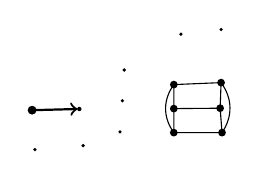
\begin{tikzpicture}[x=6mm,y=5mm]
\fill (0,0) circle (1.6pt) (1,0.03) circle (.8pt) (.06,-1) circle (.65pt) (1.08,-.9) circle (.65pt);
\draw[->,thick] (0,0)--(.96,.03);
\foreach \x/\y in {1.86/-.55,1.91/.24,1.95/1.02,3.15/1.93,4/2.05}{\fill (\x,\y) circle (.65pt);}
\draw (3,0.65)--(4,.7)--(3.98,.05)--(4.02,-.57)--(3,-.57)--cycle;
\draw (3,.04)--(3.98,.05); \draw (3,.65) to[bend right=36] (3,-.57); \draw (4,.7) to[bend left=35] (4.02,-.57);
\foreach \x/\y in {3/.65,4/.7,3/.04,3.98/.05,3/-.57,4.02/-.57}{\fill (\x,\y) circle (1.4pt);}
\end{tikzpicture}}
% archive sheet number: 104
